\section{Projektanalyse}

Im Rahmen der Projektanalyse wird der IST-Zustand ermittelt und dem SOLL-Zustand gegenübergestellt.

\begin{wrapfigure}[6]{r}[0cm]{180px}
	\vspace{-40px}
	\centering
	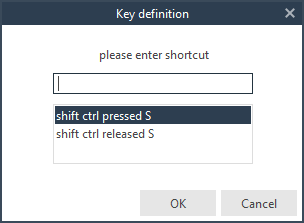
\includegraphics[width=120px]{../img/Alter-Editor.PNG}
	\caption{Bestehender Editor}
	\label{fig:existEditor}
\end{wrapfigure}

\subsection{Ist-Analyse}

Seit früheren Versionen existierte bereits ein Editor zur Eingabe von Shortcuts (siehe \autoref{fig:existEditor}). Dieser ist allerdings sehr einfach aufgebaut und beschränkt sich auf die Eingabe eines Shortcuts per Tastatur. Außerdem ist es nicht möglich Warnungen anzuzeigen oder zwischen bestehenden Shortcuts zu navigieren.

\subsection{Soll-Analyse}

Der neue Editor muss ebenfalls die Eingabe aber auch die Bearbeitung eines Shortcuts per Tastatur und Maus unterstützen. Für die Navigation und für einen besseren Überblick, werden alle bestehenden Tastenkombinationen in tabellarischen Form präsentiert. Es soll zu jedem Zeitpunkt ersichtlich sein, für welche Funktion der Shortcut definiert wird. Eine weitere Anforderung besteht darin, alle Warnungen für die entsprechenden Browser und deren Betriebssysteme anzuzeigen.

Für das Design des User Interfaces wurden von unserem UX-Designer Entwürfe angefertigt (siehe \autoref{fig:uxDesigns}). Im Designentwurf wird ersichtlich, welche Komponenten verwendet werden müssen, um alle angeforderten Informationen darzustellen und die bedarfsgerechte Bedienung zu ermöglichen.



\vfill

\begin{figure}[H] 
	\subfloat{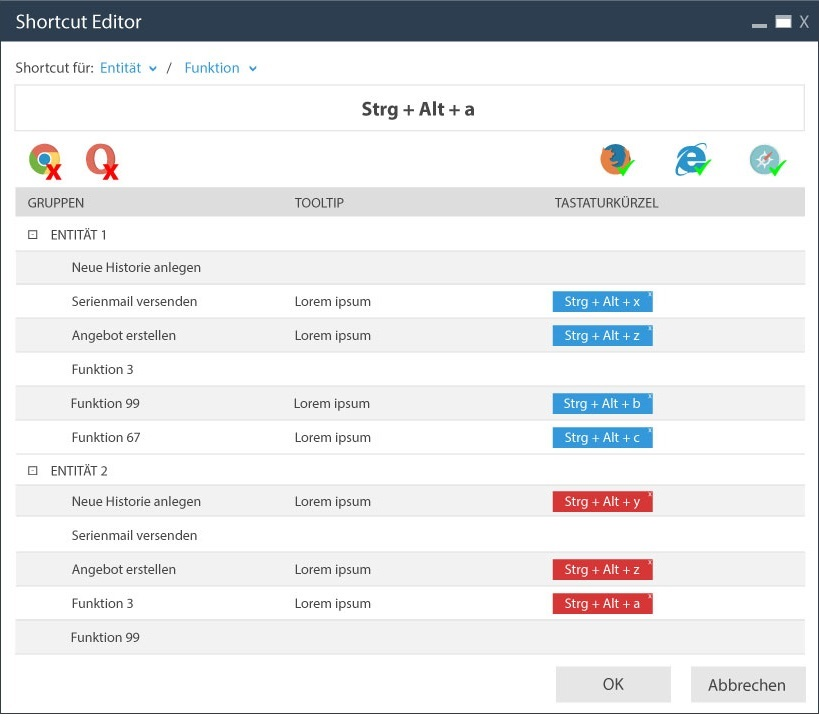
\includegraphics[width=0.5\textwidth-5px]{../img/ux/2-ShortCutEditor-Eingabe.jpg}}
	\hfill 
	\subfloat{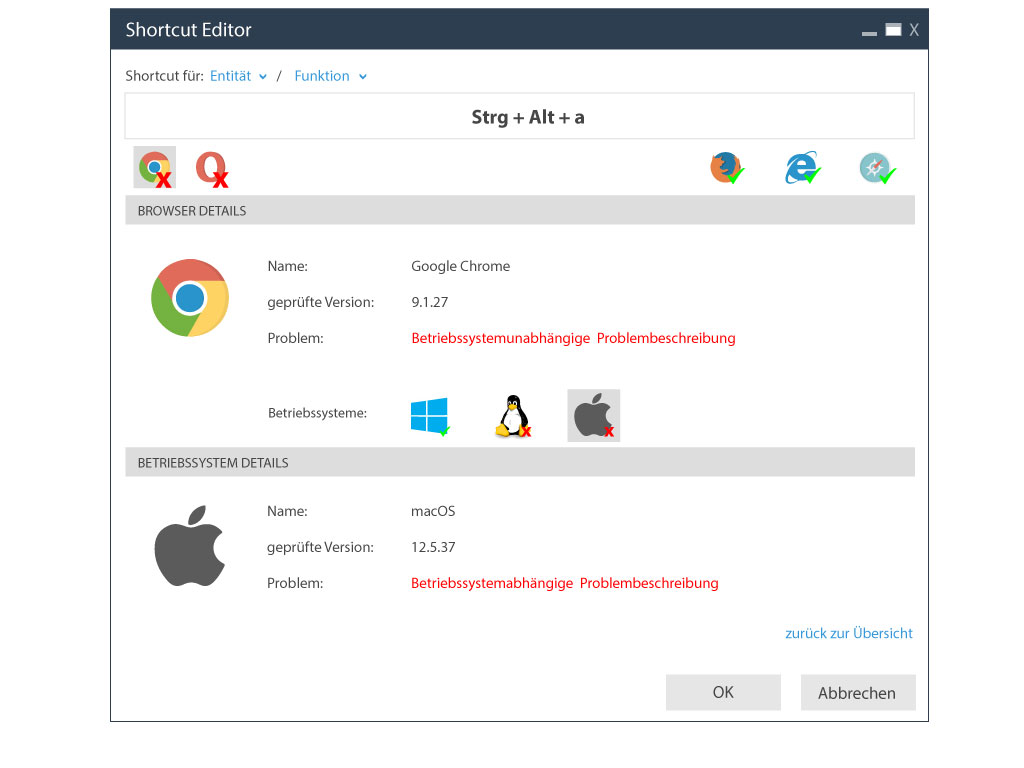
\includegraphics[width=0.5\textwidth-5px]{../img/ux/4-ShortCut-Info.jpg}}
	\caption{UI-Entwürfe der UX Abteilung} 
	\label{fig:uxDesigns}
\end{figure}

\newpage